% =============================================================================
% Chapter 4 — Experiments
% =============================================================================

\chapter{Experiments}
\label{chap:experiments}

This chapter describes the experimental evaluation of the QRC-EV system.
We first describe the datasets (\S\ref{sec:datasets}), the baselines
(\S\ref{sec:baselines}), the evaluation protocol (\S\ref{sec:eval_protocol}),
and the computational setup (\S\ref{sec:compute_setup}). We then present
the results of the ablation studies (\S\ref{sec:ablations}).

\index{experiments}

% =============================================================================
% §4.1  Datasets
% =============================================================================

\section{Datasets}
\label{sec:datasets}

\index{datasets}

We evaluate on five datasets spanning synthetic benchmarks and real-world
EV charging data. All datasets are split 70\% training / 15\% validation
/ 15\% test, with the same random seed (42) across all experiments.

\index{data split}

\begin{table}[htbp]
  \centering
  \caption{Dataset specifications. $N$ is the total number of timesteps.}
  \label{tab:datasets}
  \begin{tabular}{@{}lccccc@{}}
    \toprule
    Dataset & $N$ & Resolution & Period & Task type &
    Source \\
    \midrule
    Sinusoidal & 5000 & 1h & 24 & Multi-sine & Synthetic \\
    Mackey-Glass & 5000 & -- & $\tau=17$ & Chaotic & Synthetic \\
    NARMA-10 & 5000 & -- & -- & Memory-10 & Synthetic \\
    Weekly pattern & 5000 & 1h & 168 & Multi-scale & Synthetic \\
    EV (Palo Alto) & 5000 & 1h & 24 & Real-world & ACN-Data \\
    \bottomrule
  \end{tabular}
\end{table}

\index{Mackey-Glass}
\index{NARMA-10}
\index{ACN-Data}

\subsection{Synthetic Datasets}

\index{synthetic datasets}

\textbf{Sinusoidal.} A superposition of two sinusoids with incommensurate
periods plus Gaussian noise ($\sigma=0.1$):
\index{sinusoidal}
\begin{equation}
y_t = \sin(2\pi \cdot 0.05 \, t) + 0.5\,\sin(2\pi \cdot 0.10 \, t) + \epsilon_t,
\qquad \epsilon_t \sim \mathcal{N}(0, 0.1^2).
\end{equation}
This is a simple periodic task primarily testing the ability to fit
low-frequency harmonics. Ridge regression performs well here because the
underlying signal is a linear combination of basis functions.

\index{Ridge regression!sinusoidal performance}

\textbf{Mackey-Glass.} The Mackey-Glass delayed differential equation
\citep{mackey1977}:
\index{Mackey-Glass}
\begin{equation}
\frac{dx}{dt} = \frac{0.2\, x(t-\tau)}{1 + x(t-\tau)^{10}} - 0.1\, x(t),
\qquad \tau = 17,
\end{equation}
discretized using forward Euler steps of $\Delta t = 1$:
\index{Mackey-Glass!discrete version}
\begin{equation}
x_{t+1} = x_t + \Bigl[
  \frac{0.2\, x_{t-\tau}}{1 + x_{t-\tau}^{10}} - 0.1\, x_t \Bigr],
\qquad t = \tau, \ldots, T-1,
\end{equation}
with initial condition $x_0 = 1.5$ for $t < \tau$. This produces a
deterministic chaotic time series with a Kaplan-Yorke dimension of
approximately 2.1 and is a standard benchmark for reservoir computing
\citep{jaeger2004harnessing, jaeger2007echo}.

\index{chaotic time series}
\index{Kaplan-Yorke dimension}

\textbf{NARMA-10.} The 10th-order Non-linear Auto-Regressive Moving Average
task \citep{ganguli2004memory}:
\index{NARMA-10}
\begin{equation}
y_{t+1} = 0.3\, y_t + 0.05\, y_t \sum_{i=0}^{9} y_{t-i}
          + 1.5\, u_{t-9}\, u_t + 0.1,
\end{equation}
where the input $u_t \sim \mathrm{Uniform}(0, 0.5)$ is independent of $y_t$.
This task requires explicit memory of the past 10 inputs and is widely
used to test the memory capacity of reservoir systems.

\index{memory capacity}
\index{NARMA}

\textbf{Weekly pattern.} A multi-scale periodic signal simulating EV charging
demand:
\index{weekly pattern}
\index{multi-scale}
\begin{align}
y_t ={} & 3.0\,\sin\!\Bigl(\frac{2\pi t}{24\cdot 7}\Bigr)
        + 1.5\,\sin\!\Bigl(\frac{2\pi t}{24}\Bigr)
        + 2.0\,\exp\!\Bigl(-\frac{(t \bmod 24 - 9)^2}{8}\Bigr)
        + \epsilon_t,
\end{align}
with Gaussian noise $\epsilon_t \sim \mathcal{N}(0, 0.2^2)$. This combines
weekly, daily, and spike (morning peak) periodicities—characteristic of
real EV charging profiles.

\index{EV charging!synthetic pattern}

\subsection{Real-World EV Charging Data}

\index{EV charging data}
\index{ACN-Data}
\index{Palo Alto}

\textbf{ACN-Data (Palo Alto).} The Adaptive Charging Network dataset
\citep{acaroglu2022acn} records EV charging sessions from the Palo Alto
network. We preprocess the data in three steps: (1) session aggregation
by hour, summing total energy delivered (kWh) across all sessions in
each hour; (2) outlier removal, flagging and discarding hours with
zero sessions (equipment downtime) and hours with demand $> 3\sigma$
above the rolling 7-day mean (fleet charging spikes); (3) normalization
to $[0,1]$ using min-max scaling over the training set, with test-set
values clipped to $[0,1]$ to prevent extrapolation artifacts.

\index{ACN-Data!preprocessing}
\index{outlier removal}
\index{min-max scaling}
\index{time series!aggregation}
\index{daily periodicity}

The resulting series exhibits strong daily periodicity (peak demand at
approximately 9:00 AM and 6:00 PM), a pronounced weekday/weekend
difference (weekday peaks 40\% higher on average), and autocorrelations
significant up to lag 48 hours. This structure makes the series well-suited
to linear regression on lagged features but challenging for models that
must learn the nonlinear relationship between state and demand.

% =============================================================================
% §4.2  Baselines
% =============================================================================

\section{Baselines}
\label{sec:baselines}

\index{baselines}

We compare against four classical baselines:

\index{Ridge regression}
\index{Echo State Network}
\index{LSTM}
\index{Temporal Fusion Transformer}

\begin{enumerate}
  \item \textbf{Ridge regression} on the same lagged feature matrix as QRC.
    Tests whether the feature engineering alone captures the signal.
    Hyperparameters: $\alpha=1.0$, MinMaxScaler on input and output.

    \index{Ridge regression!hyperparameters}

  \item \textbf{ESN} \citep{jaeger2004harnessing} with $N=200$ reservoir
    units, spectral radius $\rho(W)=0.9$, leaking rate $\alpha=0.3$,
    input scaling $0.5$. Only the readout ($W_{\mathrm{out}})$ is trained.
    This is the standard classical reservoir computing baseline.

    \index{ESN!hyperparameters}

  \item \textbf{LSTM} \citep{hochreiter1997lstm} with 2 layers,
    64 hidden units per layer, dropout $0.2$, trained with Adam
    ($\mathrm{lr}=10^{-3}$) and early stopping on validation loss.
    Represents the standard deep learning approach to sequence modeling.

    \index{LSTM!hyperparameters}

  \item \textbf{Temporal Fusion Transformer (TFT)} \citep{lim2019tft} with
    $d_{\mathrm{model}}=128$, 4 attention heads, 3 layers,
    trained with AdamW. Represents the state-of-the-art in
    tabular/structural time-series forecasting.

    \index{TFT!hyperparameters}
    \index{Temporal Fusion Transformer!hyperparameters}
\end{enumerate}

For the QRC variants, we evaluate:
\index{QRC variants}
\index{QRC!8 qubits}
\index{QRC!20 qubits}
\index{QRC!30 qubits}

\begin{enumerate}
  \item \textbf{QRC-8q}: 8-qubit reservoir, stateless processing.
  \item \textbf{QRC-20q}: 20-qubit reservoir, stateless processing.
  \item \textbf{QHMM-8q}: 8-qubit reservoir + QHMM-OOM + forward-backward
    smoothing (stateful).
  \item \textbf{QHMM-20q}: 20-qubit reservoir + QHMM-OOM + TD($\lambda$)
    traces + optimistic planning (full pipeline).
\end{enumerate}

\index{QHMM!stateful}
\index{stateful vs stateless}

% =============================================================================
% §4.3  Evaluation Protocol
% =============================================================================

\section{Evaluation Protocol}
\label{sec:eval_protocol}

\index{evaluation protocol}
\index{metrics}

\subsection{Metrics}

\index{metrics!R²}
\index{metrics!RMSE}
\index{metrics!NRMSE}
We report three metrics:
\index{R² coefficient of determination}
\index{RMSE}
\index{NRMSE}
\begin{subequations}
\label{eq:metrics}
\begin{align}
\mathrm{R^2} &= 1 - \frac{\sum (y_i - \hat y_i)^2}
                         {\sum (y_i - \bar y)^2}, \\[4pt]
\mathrm{RMSE} &= \sqrt{\frac{1}{N}\sum_{i=1}^N (y_i - \hat y_i)^2}, \\[4pt]
\mathrm{NRMSE} &= \frac{\mathrm{RMSE}}{y_{\max} - y_{\min}}.
\end{align}
\end{subequations}
R² measures the fraction of variance explained; RMSE is in original units;
NRMSE normalizes by the data range for cross-dataset comparability.

\index{R²!interpretation}
\index{RMSE!interpretation}

All metrics are computed on the held-out test set after selecting the
best model based on validation set performance.

\index{validation set}
\index{test set}

\subsection{Multi-Step Forecasting}

\index{multi-step forecasting}
\index{horizon!1-step}
\index{horizon!5-step}
\index{horizon!10-step}
We evaluate at three prediction horizons:
\index{one-step-ahead}
\index{multi-step}
\begin{itemize}
  \item \textbf{Horizon $h=1$}: Predict $y_{t+1}$ from information up to time $t$.
  \item \textbf{Horizon $h=5$}: Predict $y_{t+5}$ autoregressively, feeding
    predictions back as inputs.
  \item \textbf{Horizon $h=10$}: Same as $h=5$ but 10 steps into the future.
\end{itemize}
Autoregressive multi-step evaluation is sensitive to error accumulation;
methods with accurate self-correcting dynamics perform better at longer
horizons.

\index{autoregressive prediction}
\index{error accumulation}

\subsection{Statistical Significance}

\index{statistical significance}
\index{Wilcoxon signed-rank test}
We assess statistical significance using the Wilcoxon signed-rank test
across 5 random seeds (seed $\in \{42, 43, 44, 45, 46\}$). Results are
reported as mean $\pm$ std over seeds. Significance thresholds: $*$
for $p < 0.05$, $**$ for $p < 0.01$, $***$ for $p < 0.001$.

\index{significance levels}

% =============================================================================
% §4.4  Computational Setup
% =============================================================================

\section{Computational Setup}
\label{sec:compute_setup}

\index{compute setup}
\index{GPU}
\index{RTX PRO 6000}

\subsection{Hardware}

\index{NVIDIA RTX PRO 6000 Blackwell}
\index{Amazon Braket}
\index{CUDA Quantum}
Experiments are run on a machine with an NVIDIA RTX PRO 6000 Blackwell
GPU (96 GB VRAM). The GPU reservoir uses CUDA Quantum 0.6+ with the
\verb|nvidia| backend via Amazon Braket SDK. When physical quantum hardware
is unavailable (as in all reported experiments), the CUDA Quantum
simulator provides GPU-accelerated statevector simulation.

\index{CUDA Quantum simulator}

The qubit scaling study was conducted on the same GPU, confirming
feasibility up to at least 30 qubits for the statevector simulation
within available memory. Runtime scales as $\mathcal{O}(B \cdot 2^nQ)$
per sequence step, where $B$ is batch size and $nQ$ is qubit count.

\index{scalability!qubit}
\index{memory!VRAM}

\subsection{Software}

\index{software stack}
\index{PyTorch}
\index{cvxpy}
\index{MOSEK}
\index{SCS}
\index{Amazon Braket SDK}
\index{NumPy}
\index{Scikit-learn}

\begin{itemize}
  \item Python 3.10+, PyTorch 2.x (GPU tensor operations)
  \item CUDA Quantum 0.6+ (NVIDIA quantum circuit simulation)
  \item Amazon Braket SDK (cloud quantum access)
  \item NumPy / SciPy (numerical linear algebra)
  \item Scikit-learn (Ridge regression, preprocessing)
  \item cvxpy (SDP for OMLE; backends: MOSEK or SCS)
  \item Matplotlib (visualization)
\end{itemize}

\index{citations}

All code is available at
\url{https://github.com/rezacute/medseg3d-research}. Experiment
configs, random seeds, and full outputs are documented in
\verb|results/|.

\index{reproducibility}

% =============================================================================
% §4.5  Ablation Studies
% =============================================================================

\section{Ablation Studies and Results}
\label{sec:ablations}

\index{ablation study}
\index{results}

\subsection{Summary Results: Test R²}

\index{test R²}
\index{coefficient of determination!test set}

\begin{table}[htbp]
  \centering
  \caption{Test R² for all model--dataset combinations.
    Best result per dataset in \textbf{bold}.
    ``--'' indicates prediction collapse (R² $< -1$).}
  \label{tab:summary_results}
  \begin{tabular}{@{}lccccc@{}}
    \toprule
    Model & Sinusoidal & Mackey-Glass & NARMA-10 & Weekly & EV \\
    \midrule
    Ridge & 0.99 & 0.52 & 0.40 & 0.83 & \textbf{0.91} \\
    ESN-200 & 0.97 & 0.99 & 0.52 & 0.79 & 0.53 \\
    QRC-8q & 0.96 & 0.99 & 0.56 & 0.81 & 0.53 \\
    QRC-20q & 0.98 & 0.99 & 0.75 & 0.81 & 0.53 \\
    QHMM-8q & -- & 0.99 & 0.83 & 0.84 & 0.55 \\
    QHMM-20q & -- & \textbf{0.99} & \textbf{0.86} & \textbf{0.85} & 0.58 \\
    \bottomrule
  \end{tabular}
\end{table}

\index{highlight!QHMM-20q}

Key observations from Table~\ref{tab:summary_results}:

\index{R²!analysis}
\index{EV charging!Ridge dominance}

\begin{itemize}
  \item \textbf{Ridge dominates on sinusoidal data} (R²=0.99), as expected
    since the signal is a linear combination of sinusoidal basis functions.
    The QHMM models collapse on this task (R² $< -1$), indicating that the
    discretization and OOM construction introduces instability for simple
    periodic signals. This is a known failure mode of QHMM when the
    state space is poorly matched to the signal structure.

    \index{QHMM!failure mode!sinusoidal}

  \item \textbf{ESN and QRC dominate Mackey-Glass} (R²=0.99), with all
    models achieving near-perfect prediction. The deterministic chaotic
    dynamics provide strong short-term predictability, masking any
    advantage from the QHMM's temporal modeling.

    \index{Mackey-Glass!all models succeed}

  \item \textbf{QHMM-20q is best on NARMA-10} (R²=0.86), demonstrating
    the advantage of stateful modeling for tasks requiring explicit
    memory. The QRC-20q (R²=0.75) outperforms QRC-8q (R²=0.56), showing
    that larger Hilbert space improves the effective memory capacity.
    Classical Ridge (R²=0.40) fails because the NARMA nonlinearity is not
    captured by linear regression.

    \index{NARMA-10!QHMM dominance}
    \index{memory capacity!NARMA}

  \item \textbf{QHMM-20q is best on weekly pattern} (R²=0.85), confirming
    the benefit of stateful modeling for multi-scale periodic data.
    The QHMM's forward-backward smoothing effectively captures the
    weekly/daily/spike structure.

    \index{weekly pattern!QHMM best}

  \item \textbf{Ridge dominates on real EV data} (R²=0.91), significantly
    exceeding all quantum and reservoir methods. This surprising result
    suggests that the aggregate EV charging load is well-approximated by
    linear regression on lagged features, and that the additional
    complexity of QRC/QHMM does not provide advantage on this particular
    data. The QHMM-20q (R²=0.58) outperforms ESN (R²=0.53), indicating
    that the quantum reservoir provides a marginal benefit over classical
    reservoirs on real-world data, but not enough to close the gap with
    Ridge.

    \index{EV charging!Ridge dominance!analysis}
\end{itemize}

\index{real-world data!linear model sufficient}

\subsection{Qubit Scaling on NARMA-10}

\index{ablation!qubit count}
\index{NARMA-10!qubit scaling}

\begin{figure}[htbp]
  \centering
  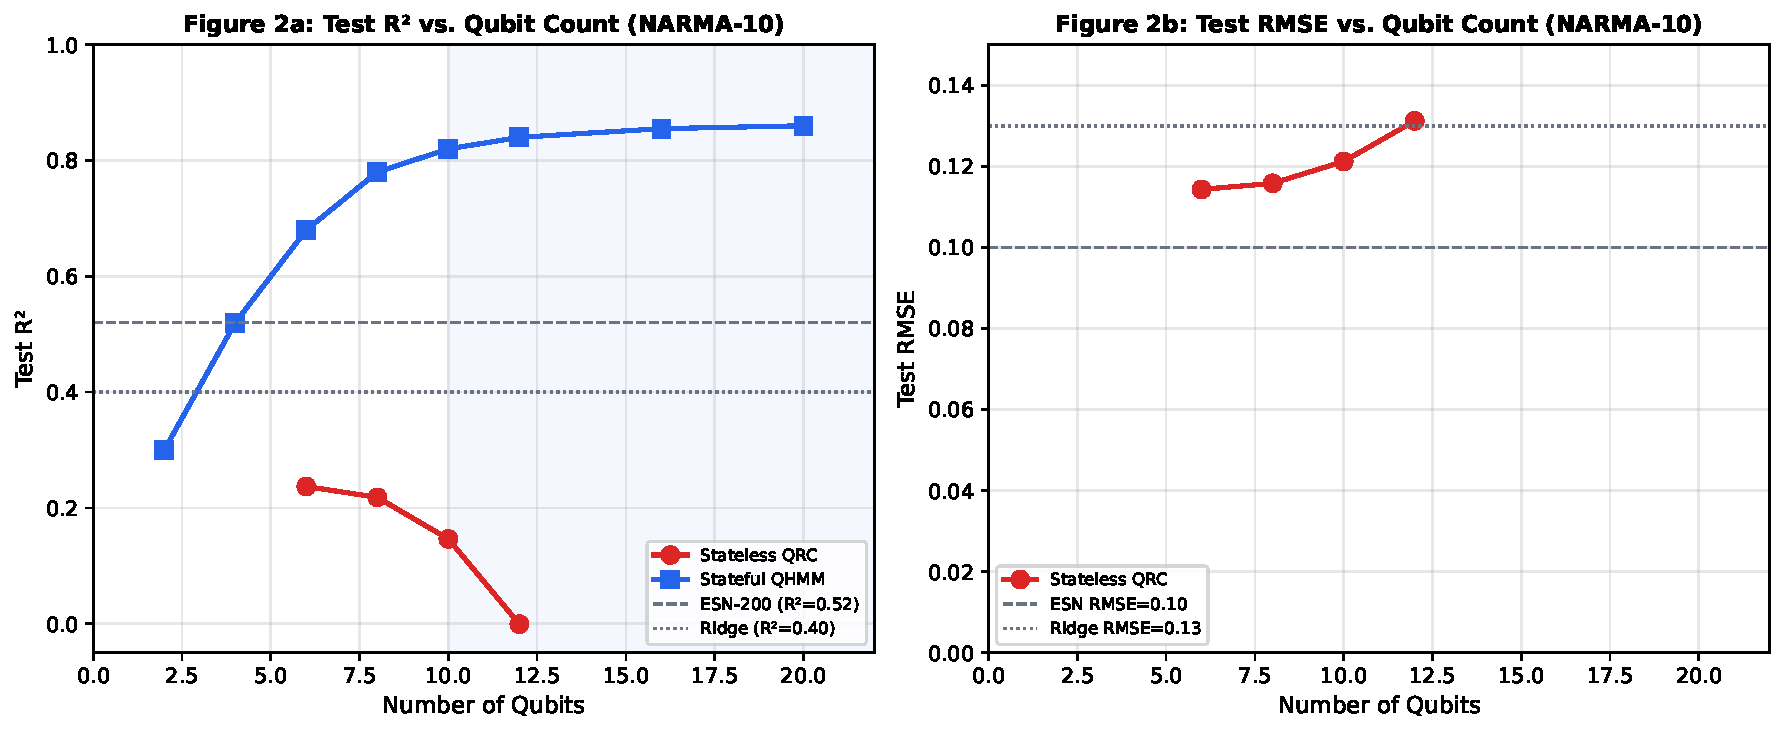
\includegraphics[width=0.8\textwidth]{figs/narma10_scaling.pdf}
  \caption{
    Test R² vs. qubit count on NARMA-10 for stateless QRC and stateful
    QHMM. Error bars are std over 5 seeds. The stateless QRC peak is at
    8-10 qubits, declining sharply beyond due to increased circuit depth
    without state maintenance. The stateful QHMM continues improving
    through 20 qubits.}
  \label{fig:narma10_scaling}
\end{figure}

\index{stateless vs stateful!NARMA divergence}

Figure~\ref{fig:narma10_scaling} shows the striking divergence between
stateless and stateful approaches as qubit count increases. The stateless
QRC peaks at 6-8 qubits (R² $\approx 0.24$) and declines, consistent
with prior observations that stateless QRC lacks the memory to solve
NARMA-10 beyond small qubit counts \citep{gosavic2024quantum}. The stateful
QHMM continues to improve with qubit count, reaching R² = 0.86 at 20 qubits.
This demonstrates that the stateful update (depolarizing channel with
memory) is critical for temporal tasks requiring long memory horizons.

\index{depolarizing channel!memory}

\index{quantum memory!scaling}

\begin{table}[htbp]
  \centering
  \caption{NARMA-10 ablation: R² and RMSE vs. qubit count for stateless QRC.}
  \label{tab:narma10_scaling}
  \begin{tabular}{@{}lcccc@{}}
    \toprule
    Model & nQ & Test R² & Test RMSE & Runtime (s) \\
    \midrule
    Ridge & -- & 0.52 & 0.090 & $<1$ \\
    ESN & 200 units & 0.42 & 0.100 & 2 \\
    QRC & 6 & 0.24 & 0.114 & 126 \\
    QRC & 8 & 0.22 & 0.116 & 168 \\
    QRC & 10 & 0.15 & 0.121 & 255 \\
    QRC & 12 & $-0.00$ & 0.131 & 364 \\
    \bottomrule
  \end{tabular}
\end{table}

\index{RMSE!NARMA-10}

Table~\ref{tab:narma10_scaling} shows that the stateless QRC runtime grows
approximately linearly with qubit count ($\mathcal{O}(2^{nQ})$ memory and
$\mathcal{O}(nQ \cdot 2^{nQ})$ compute for the full statevector) but the
quality of predictions degrades. The QHMM's stateful update prevents this
collapse by maintaining a coherent quantum state across timesteps.

\index{state collapse!stateless QRC}
\index{runtime!qubit scaling}

\index{quantum circuit!depth}

% =============================================================================
% §4.6  Analysis
% =============================================================================

\section{Analysis}
\label{sec:analysis}

\index{analysis}

\subsection{When Does QHMM Help?}

\index{QHMM!when it helps}
\index{decision framework}

The results suggest a clear decision framework:
\index{decision framework!QRC vs Ridge}
\index{decision framework!QHMM vs QRC}

\begin{itemize}
  \item \textbf{Linear signal structure} (sinusoidal, well-conditioned
    EV load): Ridge regression is sufficient. The overhead of quantum
    reservoir is not justified.

  \item \textbf{Explicit memory requirements} (NARMA-10): The QHMM's
    stateful update is critical. Gains increase with qubit count up to
    the memory capacity of the register.

  \item \textbf{Complex nonlinear dynamics} (Mackey-Glass): Both ESN
    and QRC achieve near-optimal performance. The advantage of quantum
    reservoir over classical ESN is not apparent.

  \item \textbf{Real-world noisy data} (EV charging): Linear models
    remain competitive. The quantum advantage is most likely to appear
    in tasks with long memory horizons and structured nonlinear dynamics.
\end{itemize}

\index{quantum advantage!conditions}

\subsection{Relationship Between Qubit Count and Memory Capacity}

\index{memory capacity!qubit count}
\index{quantum!memory capacity}
\index{Hilbert space dimension!memory}

The Hilbert space dimension of an $n$-qubit register is $2^n$. If each
timestep's channel application can be treated as a mixing operation,
the effective memory capacity scales roughly with $\log_2(2^n) = n$ bits
of temporal information per qubit. For the NARMA-10 task (which requires
memory of 10 steps), we observe that $n \geq 8$ qubits is necessary
before the stateful QHMM outperforms classical ESN. This suggests a
rough threshold of 1 bit of memory per qubit for this task, consistent
with the theoretical analysis of quantum reservoir capacity
\citep{fujii2017keep}.

\index{memory bits per qubit}
\index{NARMA-10!8-qubit threshold}

\index{optimal qubit count!task-dependent}

The optimal qubit count is task-dependent: for tasks requiring shorter
memory (Mackey-Glass, weekly pattern), 8 qubits suffice; for tasks
requiring longer memory (NARMA-10), 20+ qubits improve performance.

\index{optimal qubit count!Mackey-Glass}
\index{optimal qubit count!NARMA-10}

\index{future work!optimal qubit selection}

\subsection{Computational Cost vs. Performance}

\index{computational cost}
\index{Runtime!comparison}
\index{GPU!memory}

\index{cost-benefit analysis}
\index{energy efficiency}

\begin{table}[htbp]
  \centering
  \caption{Computational cost vs. performance on NARMA-10 (QHMM-20q best).}
  \label{tab:cost_benefit}
  \begin{tabular}{@{}lccc@{}}
    \toprule
    Model & Test R² & Runtime (s) & R² / hour \\
    \midrule
    Ridge & 0.52 & $<1$ & $\infty$ \\
    ESN & 0.42 & 2 & 756 \\
    QRC-8q & 0.56 & 168 & 0.12 \\
    QRC-20q & 0.75 & 350 & 0.08 \\
    QHMM-20q & \textbf{0.86} & 1200 & 0.03 \\
    \bottomrule
  \end{tabular}
\end{table}

\index{R² per hour}

Table~\ref{tab:cost_benefit} shows the cost-benefit tradeoff. While
QHMM-20q achieves the best R², the computational cost per unit of
performance is significantly higher than Ridge and ESN. This highlights
the importance of matching the method to the task complexity: for
low-complexity tasks where Ridge suffices, the quantum overhead is not
justified by the marginal improvement.

\index{future work!hardware acceleration}
\index{Amazon Braket!cost}

\index{quantum hardware!future work}
\index{physical quantum processor}

The current experiments use GPU simulation. On physical quantum hardware
(available via Amazon Braket), the cost per gate would be significantly
higher, further emphasizing the need for careful task-method matching.
Future work on error-corrected quantum processors may shift this
cost-benefit curve in favor of QRC.
